\documentclass[a4paper]{article}

\usepackage{fullpage}
\usepackage{listings}
\usepackage{url}
\usepackage{forest}
\usepackage{graphicx}

\definecolor{folderbg}{RGB}{124,166,198}
\definecolor{folderborder}{RGB}{110,144,169}

\def\Size{4pt}
\tikzset{
  folder/.pic={
    \filldraw[draw=folderborder,top color=folderbg!50,bottom color=folderbg]
      (-1.05*\Size,0.2\Size+5pt) rectangle ++(.75*\Size,-0.2\Size-5pt);  
    \filldraw[draw=folderborder,top color=folderbg!50,bottom color=folderbg]
      (-1.15*\Size,-\Size) rectangle (1.15*\Size,\Size);
  }
}

\begin{document}

\title{\Huge\bfseries Robot Simulator, v180107}
\date{7th January, 2018}

\maketitle

\tableofcontents

\section{A Word of Caution}

Simulators, by their very nature, are approximations of the real
world. Various approximations are made to develop them and, as a
result they do not model the world perfectly. Therefore, they should
be treated as an {\itshape aid\/} to the development of your
system. It does not replace working with the actual robotic platform.

\section{Version History}

\begin{itemize}
\item {\bfseries 160430}: Initial release
\item {\bfseries 160505}: Include methods for custom setting of
  encoder ticks.
\item {\bfseries 170108}: Significant rewrite of geometry handling to
  support collision of wheels with walls. Support wall material
  types. Added multiple IR sensor detection profiles which are chosen
  randomly. Inject random noise into robot movement. Approximate
  maximum acceleration constraints.
\item {\bfseries 170123}: Added trails which robots can leave in the
  environment. Added macros to show if the code is being built in the
  simulator or not. Updated instructions to remove some errors.
 \item {\bfseries 180107}: Made configuration of IR sensors externally
 controllable through log files. Added ability to show sensor firing in the GUI.
\end{itemize}

\section{Prerequisites}

The simulator has been tested to work on Ubuntu Linux 16.04, macOS High Sierra
and Windows 10, 64-bit edition but is likely to work on many other combinations
of operating system and build environments. For example, it has been used in the
Windows Subsystem for Linux. It uses standard software with no third party
dependencies.

The project files consist of a large number of small programs which mostly
communicate by writing messages to a console. Such programs tend to be very
inefficiently managed using IDEs. Therefore, we do \emph{not\/} recommend the
use of any IDE such as Developer Studio or XCode but, rather, to use command
line tools directly. In addition, command line is used quite often as a fallback
in many, many systems, and having a familiarity with it is very useful in its
own right.

\begin{itemize}
\item {\bfseries Windows:} The recommended system to use is
  cygwin. The installer can be downloaded from
  \url{https://www.cygwin.com/}. You should install the cmake, make
  and g++ packages.
\item {\bfseries macOS:} The shell (bash) and the compiler (clang)
  come with the system (although you might have to install the Xcode
  command line tools). For package management, it is highly
  recommended that you use homebrew to install the basic system
  libraries (\url{http://brew.sh/}) together with cask
  (\url{https://caskroom.github.io/}) to manage installing
  applications.
\item {\bfseries Linux:} The command line tools are already provided,
  and only the below requirements need to be met.
\end{itemize}

To run the simulator, you will need:

\begin{itemize}
\item Java JRE 1.8 or above, \url{https://java.com/en/download/}.
\item A C++11 or above compliant compiler, including gcc and
  clang.
\item CMake, version 2.8.4 or above. This can be obtained from
  \url{https://cmake.org/download/}.
\end{itemize}

Optionally, you can install Eclipse
(\url{https://eclipse.org/downloads/}) Neon (or above) to use the
project files to build the simulator.

\section{Package Structure}

Uncompress the zip file to give the following directory structure:

\begin{forest}
  for tree={
    font=\ttfamily,
    grow'=0,
    child anchor=west,
    parent anchor=south,
    anchor=west,
    calign=first,
    inner xsep=7pt,
    edge path={
      \noexpand\path [draw, \forestoption{edge}]
      (!u.south west) +(7.5pt,0) |- (.child anchor) pic {folder} \forestoption{edge label};
    },
    before typesetting nodes={
      if n=1
        {insert before={[,phantom]}}
        {}
    },
    fit=band,
    before computing xy={l=15pt},
  }  
[robotsimulator
  [Client
    [applications
    ]
    [Examples
    ]
    [include
    ]
    [src
    ]
    [tests
    ]
  ]
  [Documentation
  ]
  [Simulator
  [bin
  ]
  [lib
  ]
  [maps
  ]
  [robot\_params
  ]
  [src
  ]
]
]
\end{forest}

\subsection{Simulator}

This was built using Java in Eclipse. The full Eclipse project is included, but
a precompiled, runnable jar file (\verb+Simulator/bin/simulator.jar+) is shipped
so that no building is required. Therefore, you should be able to double
click on it to run. You might need to give it permission to act as a server in a
firewall.

\subsection{Client}

Unlike the server, the client is in C / C++ code and must be built on the local
operating system / build environment. The client consists of a library,
\verb+libclient+, which includes a networking library
(\verb+Client/src/Practical_Socket+), a library for linking with the simulation
(\verb+Client/src/Client+) and a port of a number of the standard Propeller IDE
libraries (in \verb+Client/src/Simple_Libraries+).

The meta-build system \verb+cmake+ (\url{https://cmake.org/}) is used.
\verb+cmake+ uses high-level text files to specify a project. It can use these
to generate build systems for a huge range of development platforms (including
makefiles, Visual Studio solutions, nmake makefiles, Xcode projects, and eclipse
workspaces) for a huge range of platforms (including OSX, Linux, Windows, and
Cygwin under Windows).

\subsubsection{Build Instructions}

For all platforms, command line building is the recommended approach. The
command is

\begin{verbatim}
cmake SOURCE_DIRECTORY
\end{verbatim}

If you are compiling within the source directory, you would use:

\begin{verbatim}
cmake .
\end{verbatim}

(Note the ``.'' to mean current directory.)

You should see the following. (Note that \verb+Hnatt:Client ucacsjj$+ is the
command line prompt generated by my machine and shows the machine name,
directory and user. Your prompt will be different.)

\begin{verbatim}
Hnatt:Client ucacsjj$ cmake .
-- Looking for pthread.h
-- Looking for pthread.h - found
-- Looking for pthread_create
-- Looking for pthread_create - found
-- Found Threads: TRUE  
-- Configuring done
-- Generating done
-- Build files have been written to: /Users/ucacsjj/Proj/Simulator/Code/Trunk/Source/Client
\end{verbatim}

The code can then be built using:

\begin{verbatim}
make
\end{verbatim}

You should then see something like:

\begin{verbatim}
Hnatt:Client ucacsjj$ make
[  1%] Building CXX object src/CMakeFiles/client.dir/Practical_Socket/PracticalSocket.cpp.o
[  1%] Building CXX object src/CMakeFiles/client.dir/Client/Console.cpp.o
[  1%] Building CXX object src/CMakeFiles/client.dir/Client/ServerConnection.cpp.o
[  2%] Building CXX object src/CMakeFiles/client.dir/Client/launcher.cpp.o
[  2%] Building CXX object src/CMakeFiles/client.dir/Client/simulator.cpp.o
[  3%] Building CXX object src/CMakeFiles/client.dir/Simple_Libraries/Motor/libservo/servo.cpp.o
[  3%] Building CXX object src/CMakeFiles/client.dir/Simple_Libraries/PropellerGCC/cog.cpp.o
[  4%] Building CXX object src/CMakeFiles/client.dir/Simple_Libraries/PropellerGCC/CogManager.cpp.o

....

[100%] Linking CXX executable Cog_Info_Exchange
[100%] Built target Cog_Info_Exchange
[100%] Building C object applications/CMakeFiles/spinLeftRight.dir/spinLeftRight.c.o
[100%] Linking CXX executable spinLeftRight

\end{verbatim}

You may see a number of warnings. These can be safely ignored. They
occur because of the way in which the programs are wrapped so that
they look the same both in the robot and in the simulator.

\section{Usage}

\subsection{Simulator}

For the simulator, simply double click on the jar file to open. This should
present you with the window:

\begin{center}
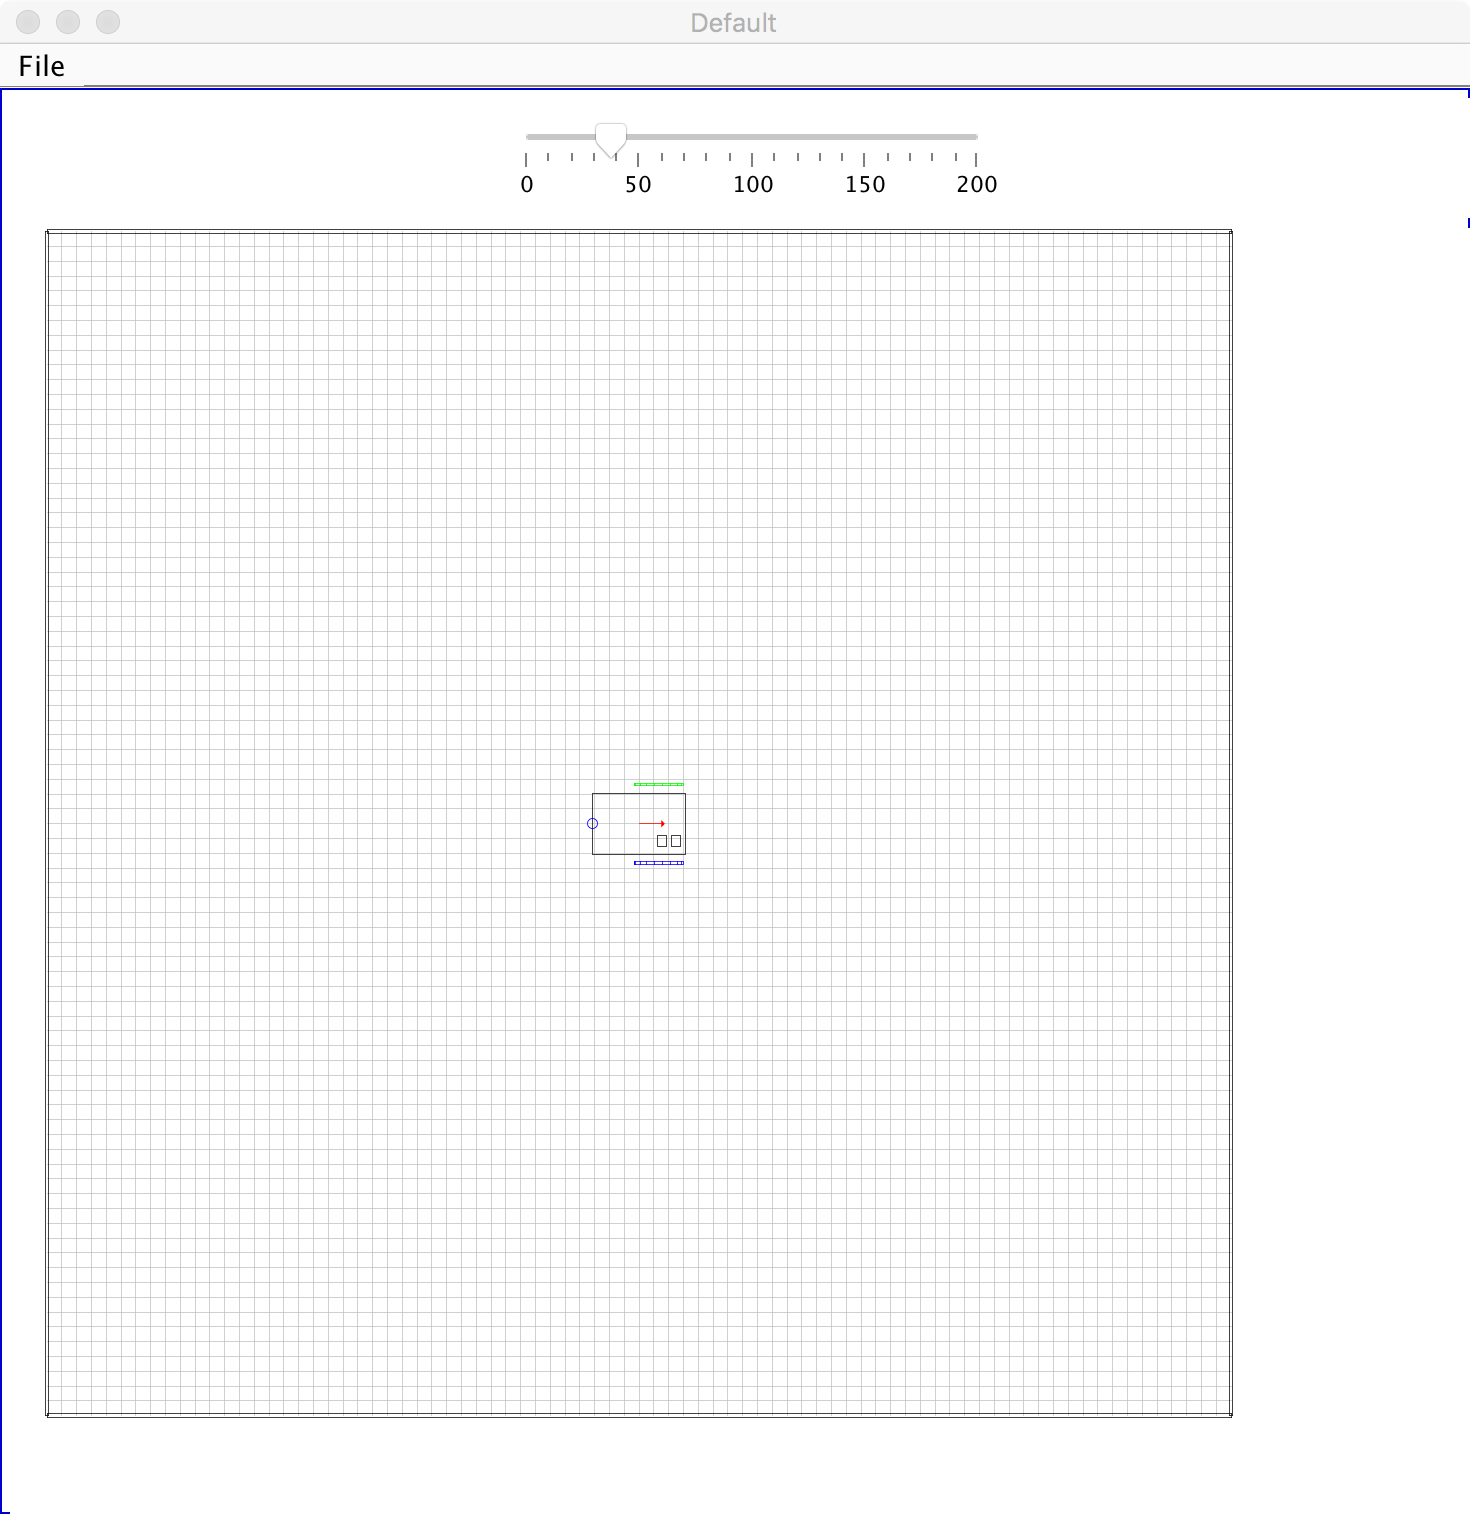
\includegraphics[width=0.5\linewidth]{default_scenario.png}
\end{center}

The GUI options are (deliberately) very simple. The slider only
changes the zoom setting (the mousewheel or equivalent can be used to
zoom in and out).

The \verb+File+ menu supports loading a map from file, refreshing a
map (which reloads a previous specified map) or exiting.

The maps are all in the \verb+Simulator/maps+ directory. The figure
below shows the map obtained from loading Maze 02:

\begin{center}
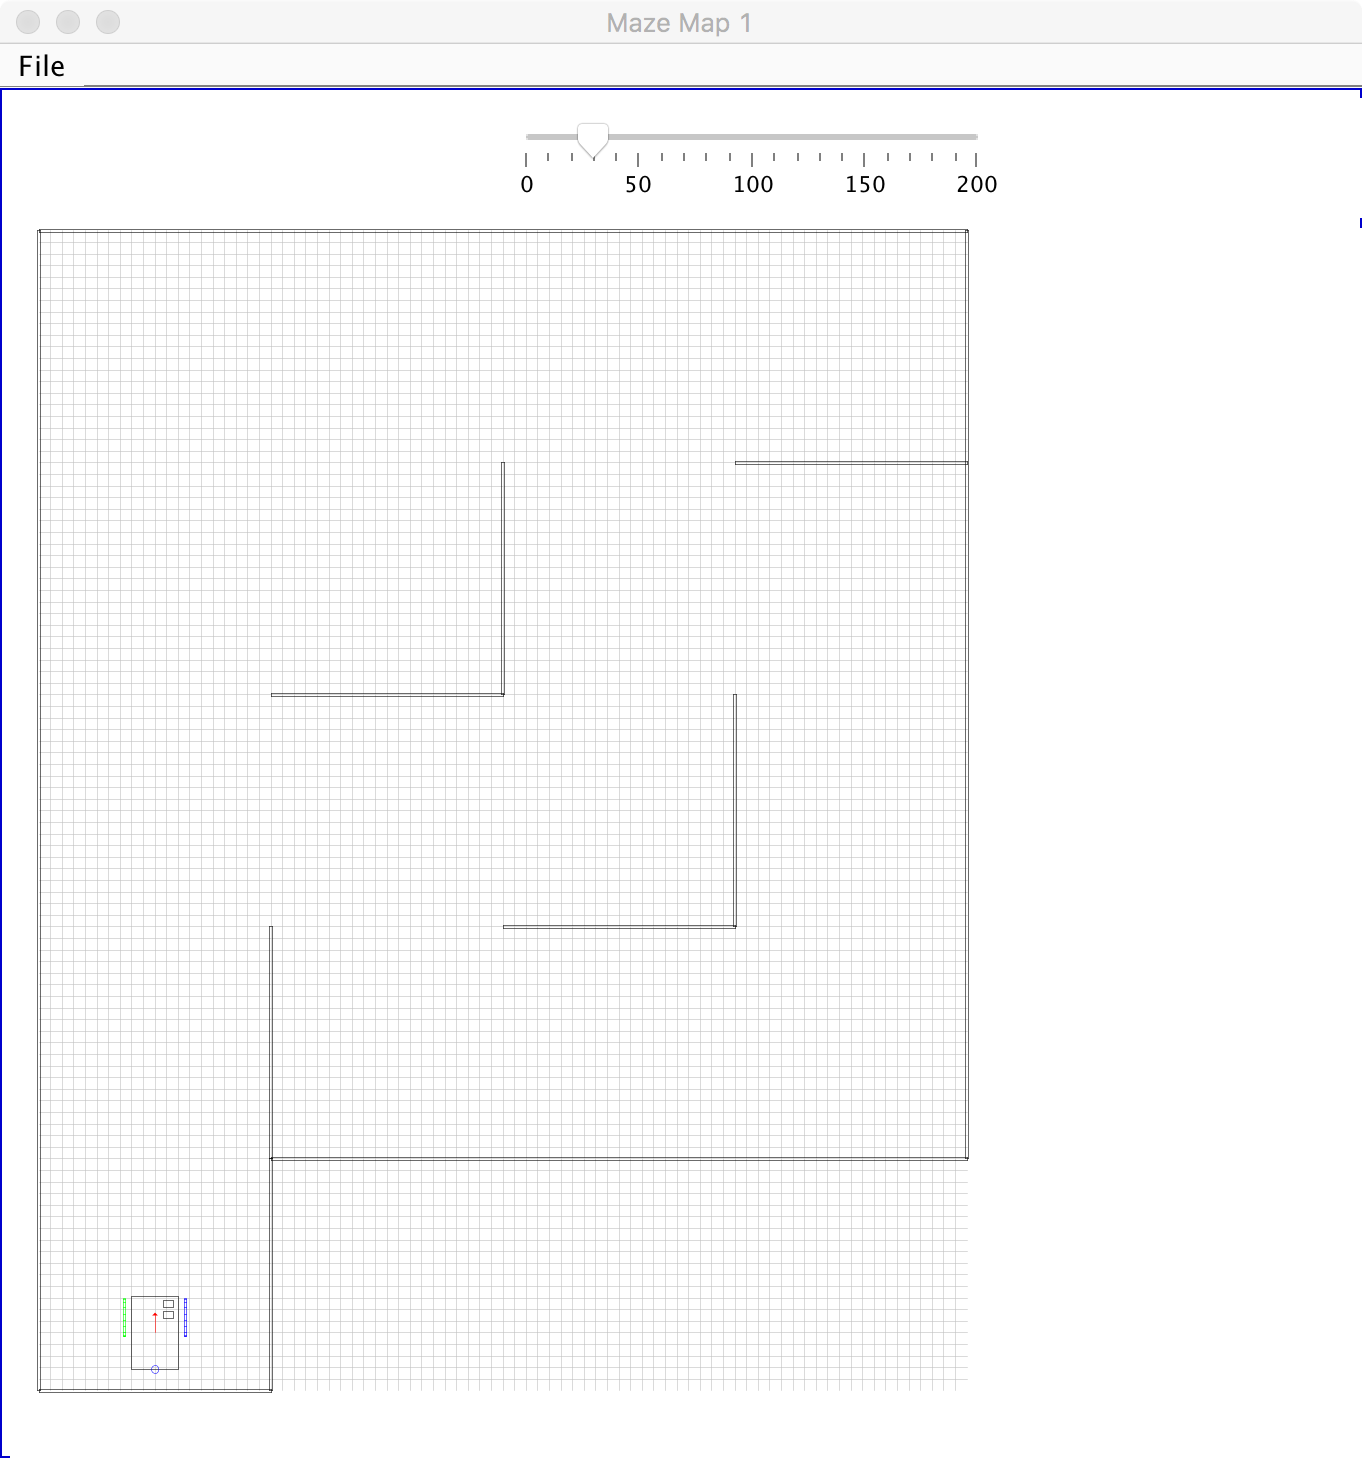
\includegraphics[width=0.5\linewidth]{Maze_Map01.png}
\end{center}

The map files are stored using a JSON format. The format should be
``self-explanatory'' but, if people are interested, documentation on it can be
provided.

The graphics will show, in real time, the firing of the sensors as well. The
ping sensor is shown as a ray which faces towards the front, and the IR sensors
are rays to the left and right.

\subsection{Client}

Any program you build will be linked into a command line
application. You should be able to build most applications ``out of
the box'' without any modification. (The only requirement is that
\verb+simpletools.h+ \emph{must\/} be included by the file which
includes the declaration of the \verb+main+ function.)

For example, consider the contents of
\verb+Client/tests/testDriveSpeed.c+:

\lstset{language=C++} 

\begin{verbatim}
#include <stdio.h>
#include <stdlib.h>
#include <time.h>

#include "abdrive.h"
#include "simpletext.h"
#include "simpletools.h"
#include "ping.h"

int main(int argc, const char* argv[])
{
  // Drive ahead nice and slow
  drive_speed(16, 16);

  struct timeval tv;
  
  gettimeofday(&tv, NULL);

  long int startSecs = tv.tv_sec;
  
  while(ping_cm(8) > 8)
    {
      pause(100);
      struct timeval now;
      gettimeofday(&now, NULL);
      if (now.tv_sec != tv.tv_sec)
        {
          int left, right;
          drive_getTicks(&left, &right);
          printf("%ld %d %d\n", now.tv_sec-startSecs, left, right);
          tv.tv_sec = now.tv_sec;
        }
    }
}
\end{verbatim}

This program sets up the drive speed so that the robot slowly trundles forwards
and, once per second, prints out the drive ticks (the encoder values in the
wheels which say how far a wheel has turned).

The client library can issue messages. These are formatted as
\verb+[library] method(line): <<MESSAGE>>+.

If the client cannot connect to the server, you'll see a message like:

\begin{verbatim}
Hnatt:Client ucacsjj$ ./tests/testDriveSpeed 
[PropGCC] start(28): start: Initialised with 8 available cogs
[libsimpletools] LibSimpleToolsStarter(19): Time ticks setup
[libsimpletools] LibSimpleToolsStarter(20): ms=80000
[libsimpletools] LibSimpleToolsStarter(21): us=80
[libsimpletools] LibSimpleToolsStarter(22): st_iodt=80
[libsimpletools] LibSimpleToolsStarter(23): st_pauseTicks=80000
[libsimpletools] LibSimpleToolsStarter(24): st_timeout=20000000
[libsimpletool] eepromStart(15): eepromStart: Setting up EEPROM with 65536 bytes
[libsimpletool] eepromStart(16): eepromStart: EEPROM is simulated using an in memory buffer
 and is not persistent
[simpletext] LibSimpleTextStarter(30): Started with stdio stubs for the simpleterm
[ServerConnection] open(57): Could not open connection with the simulator - is it running?
[PropGCC] stop(14): stop: Joining all cog threads; might hang
\end{verbatim}

If the connection is successful, the output will be:

\begin{verbatim}
[PropGCC] start(28): start: Initialised with 8 available cogs
[libsimpletools] LibSimpleToolsStarter(19): Time ticks setup
[libsimpletools] LibSimpleToolsStarter(20): ms=80000
[libsimpletools] LibSimpleToolsStarter(21): us=80
[libsimpletools] LibSimpleToolsStarter(22): st_iodt=80
[libsimpletools] LibSimpleToolsStarter(23): st_pauseTicks=80000
[libsimpletools] LibSimpleToolsStarter(24): st_timeout=20000000
[libsimpletool] eepromStart(15): eepromStart: Setting up EEPROM with 65536 bytes
[libsimpletool] eepromStart(16): eepromStart: EEPROM is simulated using an in memory buffer
 and is not persistent
[simpletext] LibSimpleTextStarter(30): Started with stdio stubs for the simpleterm
[ServerConnection] getRobotHandle(92): The robot handle is 0
[simulator] simulator_showRobotConfiguration(110): simulator_showRobotConfiguration The returned robot configuration is:
...
\end{verbatim}

The robot configuration specifies details about how the robot is set up. If
there are problems --- for example with the IR sensors not working properly ---
you should make a note of this information when talking with the TAs.

Note that not all functions have been implemented. One example is the
function \verb+dac_ctr_stop()+, which does nothing in the
simulator. If you call it, you will see a message of the form:

\begin{verbatim}
[abdrive] dac_ctr_stop(43): dac_ctr_stop stub implementation
\end{verbatim}

\subsection{Writing Your Own Applications}

There are two issues to consider:
\begin{enumerate}
\item Creating a new directory for applications.
\item Creating a new application in an existing directory.
\end{enumerate}

These are slightly different because when you create a new directory,
\verb+cmake+ has to be made aware that the directory is there.

\subsubsection{Creating a New Directory}

Suppose you want to create a new directory \verb+Task1+ in the
\verb+applications+ subdirectory. There are four steps:

\begin{enumerate}
\item Create the directory \verb+Task1+ in \verb+applications+
\item Modify the CMakeLists.txt file in \verb+applications+ and add the line
  \begin{verbatim}
    ADD_SUBDIRECTORY(Task1)
  \end{verbatim}
\item Create a CMakeLists.txt file in \verb+Task1+. See the second
  below on how to declare a new application.
\item Run cmake \emph{once\/} from the \verb+applications+ directory.
\end{enumerate}

When this happens, cmake notices that \verb+CMakeLists.txt+ has
changed, and loads the new version. It then sees that there is a new
directory (\verb+Task1+) and stores that this directory needs to be
checked in the future. It also loads \verb+Task1/CMakeLists.txt+ and
does whatever processing is required.

After this, it is sufficient to just cd into the \verb+Task1+
directory and run \verb+make+. The dependency system will now pick up
if, for example, you create a new application and will update everything automatically.

\subsubsection{Creating a New Application in an Existing Directory}

If the directory has been registered, you create a new application by
adding a line of the form \verb+DECLARE_APP(appName sourceFiles)+. For
example, suppose you wanted to build an application called
\verb+testDrive+ and it had one source file called
\verb+my_test_drive_code.c+. The syntax would be:
\begin{verbatim}
DECLARE_APP(testDrive my_test_drive_code.c)
\end{verbatim}

If you have several files --- for example a common library file. These
are just added as well. For example, if in this example we also had
the file \verb+my_common_tools.c+, then the declaration would be
changed to:
\begin{verbatim}
DECLARE_APP(testDrive my_test_drive_code.c my_common_tools.c)
\end{verbatim}

\subsubsection{Writing Code Which is Only Used in the Simulator}

The simulator provides a few special ``extended'' commands such as
drawing trails and rescaling the resolution of the encoders. These are
\emph{not\/} available in the ActivityBot API --- if you use these
directly your code will not compile.  To prevent this from happening,
the simulator defines the C macro \verb+BUILDING_IN_SIMULATOR+. An
example usage is as follows. This includes the file \verb+simulator.h+
and runs the start trail command on the simulator.

\begin{verbatim}

#include "abdrive.h"
#include "simpletext.h"
#include "simpletools.h"

#ifdef BUILDING_IN_SIMULATOR
#include "simulator.h"
#endif

int main(int argc, const char* argv[])
{
#ifdef BUILDING_IN_SIMULATOR
  simulator_startNewSmokeTrail();
#endif
 drive_goto(100, 100);
#ifdef BUILDING_IN_SIMULATOR
  simulator_stopSmokeTrail();
#endif
  return 0;
}

\end{verbatim}

\subsection{Interesting Facts and Limitations}

\begin{enumerate}
\item {\bfseries Simulation Time vs. Real Time:} The simulator
  attempts to accurately simulate the temporal sequence of
  activites. For example, the pause in the return of a measurement
  from a \verb+ping+ request depends on how far a target is from the
  robot. To model this timing accurately, the simulator has its own
  simulation time. This typically runs at half real-time but, in some
  operations can be slower. This will be obvious as the robot
  appearing to ``speed up'' and ``slow down'' in the GUI. However, all
  method associated with reporting system time will report the
  simulation time and so these effects should not be evident.
\item {\bfseries EEPROM:} The Propeller Board has an EEPROM which can
  act as a persistent store. Data can be written to --- and read from
  --- this store. It is often used to store wheel calibration
  data. The simulator simulates the EEPROM but the storage is not
  persistent. If the program exits, the data stored in EEPROM is lost
  as well. If you wish the simulator to simulate persistency in the
  EEPROM, let us know and we will attempt to implement it.
\item {\bfseries Cogs:} The Propeller Board has a set of eight
  ``cores'' or ``cogs'' which can run separately and in parallel. The
  simulator emulates these using threadings. However, there are two
  important limitations. First, in the simulator, only a single thread
  can query the simulation server at a time. Therefore, asynchronous
  operation cannot be supported. Second, cogs have termination
  semantics different from threads. The cog termination routines when
  translated to C++ thread termination semantics cause programs to
  abort. Therefore, use of cogs in the simulator is highly
  discouraged.
\end{enumerate}

\end{document}
